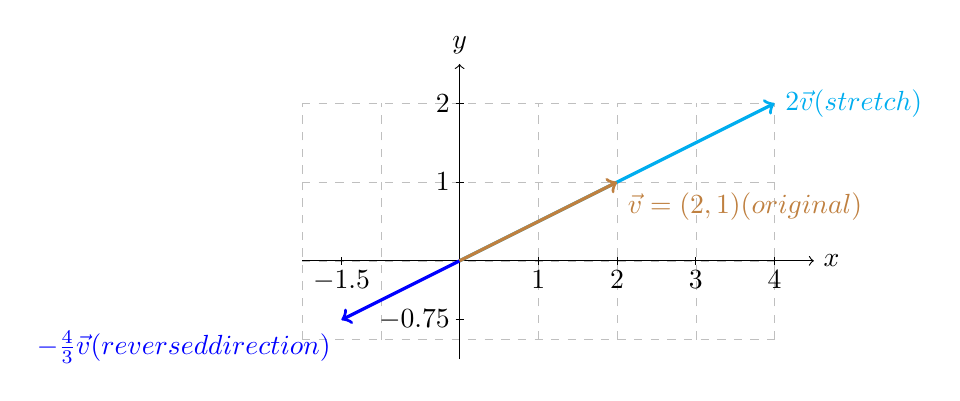
\begin{tikzpicture}
    \draw[step=1,help lines, dashed,lightgray] (-2,-1) grid (4,2);
    %draw axis value
    \foreach \x in {-1.5,1,2,3,4}
        {%
            \draw (\x,0) -- (\x,0) node [below] {$\x$};
            \draw [-] (\x,-0.05) -- (\x,0.05) ;
        }
    \foreach \y in {-0.75,1,2}
        {%
            \draw (0,\y) -- (0,\y) node [left] {$\y$};
            \draw [-] (-0.05,\y) -- (0.05,\y) ;
        }
    %draw lines
    \draw [->] (-2,0) -- (4.5,0) node[right]{$x$};
    \draw [->] (0,-1.25) -- (0,2.5) node[above]{$y$};
    \draw [<-,blue,very thick] (-1.5,-0.75) node[below left]{$-\frac{4}{3}\vec{v}(reversed direction)$} -- (0,0);
    \draw [->,cyan,very thick] (0,0) -- (4,2) node[right]{$2\vec{v}(stretch)$};
    \draw [->,brown,very thick] (0,0) -- (2,1) node[below right]{$\vec{v}=(2,1)(original)$};
\end{tikzpicture}
\captionof{figure}{{\footnotesize scalar multiplication}}
\label{fig:vector-and-vector-operation-d9}
